\documentclass[a4paper,11pt]{article}

\usepackage{fullpage}
\usepackage{amsmath}
\usepackage{amsfonts}
\usepackage{graphicx}
\usepackage{subfigure}
\usepackage{color}
\usepackage{hyperref}
\usepackage{url}

\newcommand{\todo}[1]{\textcolor{red}{\sc #1}}

\title{[MIR] Object Tracking Lab Report}

\author{Gijs Molenaar, Arjan Nusselder\\
\{gmolenaa,anussel\}@science.uva.nl}

\date{\today}

\begin{document}

\maketitle

\abstract{Object tracking in moving images is an important area of research. To get acquainted with this field, we implemented and evaluated an object tracker using the mean-shift algorithm on colour-based features. It appears that mean-shift is indeed better than an (optimised) exhaustive search approach. Different colour spaces each have their merit, as do histogram size and scaling, but no clear best performance can be pointed out. Possible improvements include automating colour space choice and handling lost objects.}


\section{Introduction}
\label{sec:introduction}
With the amount of available video footage nowadays, the need for automated analysis becomes more pressing.
Many typical applications of such analysis exist, one of which is object tracking.
Visual object tracking in general requires the identification of an object and the tracking of movement over time.
To this end, several well known algorithms exist, including kernel-based methods.
Although these algorithms have been studied before, object tracking is not yet considered a `solved problem'.

In this report we consider the mean-shift algorithm, a kernel-based method, and do a comparitive analysis with respect to colour spaces and complexity in different video domains.
We extend this analysis with a focus on the specific problems of object occlusion and scaling.

First an overview is given of the theory (section \ref{sec:theory}) and the data we used for analysis (section \ref{sec:data}).
Second we detail the application of the theory to the data, and discuss any problems we encountered (section \ref{sec:application}).
Some specific implementation details are noted in section \ref{sec:application:implementation}.
Third we evaluate and compare different aspects of the application in section \ref{sec:evaluation}, and give an interpretation of the results in section \ref{sec:results}.
Last we try to come to a conclusion about the current results and discuss possible improvements in section \ref{sec:discussion}.


\section{Theory}
\label{sec:theory}
In the current project, tracking is done on a preset sequence of still images.
There are two main problems that need to be solved.
First it is necessary to interpret a single image, in terms of the object present therein.
Second two consecutive images, or frames, must be compared to find changes between the two.
The two problems can combined into one solution using colour spaces as a feature of representation and comparison.
Below are detailed descriptions of the theory that the implementation is based upon.

\subsection{Colour Spaces}
\label{sec:theory:colour}
It is assumed that in most cases the original input will be in RGB.
This RGB model describes colour as an addition of three primary components --red, green and blue-- with respect to some spectral definition.
Each point in an image (a pixel) can then be described as a combination of these values.
Small changes in the shot conditions however, also cause these absolute colour values to change.
As such, RGB is not very robust against for instance illumination or geometrical changes.
Two other colour models, that can both be derived from RGB, were used for the current system.\cite{surveycolor}

Normalised RGB (rgb) is a model where each colour value is divided by the sum of all three colour values:
\begin{equation}
\label{eq:rgb}
r = \frac{R}{R+G+B},\; g = \frac{G}{R+G+B},\; b = \frac{B}{R+G+B}
\end{equation}
As with RGB, it describes a point as a combination of three colour components.
However, when the actual colours in an image change but all R, G and B values change proportional to each other, then the r, g and b values will not change.
This makes rgb a useful feature that is robust against normal illumination changes and other proportional colour changes like viewpoint and shape deformation.
A problem still exists with the extremities of illumination where there is hardly any colour, for example with darkness or highlights.

The hue, saturation and intensity (HSI) model uses a different kind a representation.
Now the three components each describe a property of the colour rather than a combinatory value.
Hue defines the dominant spectral colour of the source.
Saturation describes \emph{how} dominant this spectral colour is with respect to the rest of the (visible) spectrum.
Intensity is the total spectral energy (brightness) of the source.

Normally objects will effect the same hue if the colour of the light source illuminating a scene does not change.
This makes hue a usable single-valued feature that has the same robustness as rgb, with the added benifit of better handling highlights.
Hue can be derived from RGB using equation \ref{eq:hue}.

\begin{equation}
\label{eq:hue}
H = arctan\left(\frac{\sqrt{3}\,(G-B)}{(R-G)+(R-B)}\right)
\end{equation}

\subsection{Histograms}
\label{sec:theory:histograms}
In its simplest form, creating a histogram is just counting the number of times each value occurs in a given set.
In this case the histogram of a set of pixels is needed, typically a subset of all pixels in an image.
The values of a pixel are those derived from the colour features as described in section \ref{sec:theory:colour}.

Because there are many different values possible, often the size of the bins in a histogram is increased.
This way, nearby pixel-values are presented as an instance of a single bin-value.
Having larger bins directly results in a fewer number of different bins.
This can make calculations based on histograms much more computationally tractable.
It is also a simple way of generalizing, having similar colours represented as one, albeit with arbitrary borders.
Such a generalisation can reduce some of the effects that textures can have on an object.
On the downside, this does decrease the ability of the histogram to distinguish between subtle colour differences.
As long as objects in an image, which are the main focus in this report, are clearly separated from the background and have a more or less uniform colour, this is not a big problem.

With the histogram and the original image, it is then possible to do a backprojection.
For each pixel in the image, the histogram-value of its colour is retrieved and placed in a backprojection image equal in size to the original image.
If viewed as a grey-scale image, the backprojection highlights the dominant colour regions of the original image and serves as a mask for the object within this image.
Object recognition in novel images can also be done.
Using the histogram of a target image, the entire new image can be converted to a backprojection.
Regions with a high histogram-value can then be identified in this new image, and labeled as a likely instance of the original object.

\subsubsection{Epanechnikov}
\label{sec:theory:epanechnikoc}
A reasonable assumption is that the main part of the object is always in the centre of the set of pixels.
Rather than using a standard uniform kernel, it is also possible to weigh the pixels in an image according to their position.
One such kernel is the Epanechnikov kernel.
This kernel assigns a higher weight to the pixels in the centre of an image.
Instead of adding $1$ to each bin, we now add a weighted amount, based on a pixels' distance to the centre ($x$) and the Epanechnikov kernel, according to equation \ref{eq:epanechnikov}.

\begin{equation}
\label{eq:epanechnikov}
w = \left\{ \begin{array}{cl}
  \frac{4}{2\pi} (1-x^2) & \textrm{if } x \in [0,1]\\
  0 & \textrm{otherwise} \end{array}\right.
\end{equation}

Implicitly the Epanechnikov kernel also introduces a separation of background and foreground, because colours in the centre of the tracked area, belonging to the object, receive a higher weighting than the outer areas.
This also increases the dependency (bias) on the initial selection of the object \emph{area}.

\subsection{Distance Measures}
\label{sec:theory:distance}
Object tracking requires the comparison of the two parts of images in consecutive frames.
This comparison can be done with the histograms of these images --or sets of pixels-- given that the histograms are of equal form: the same colour features must be used in both cases, with an equal number of bins.
Next a distance measure must be defined that projects the two histograms to one single distance value.
When histograms are compared, a distance measure can be said to calculate how much alike they are.

A simple measure is the Euclidian distance.
In this measure, each bin is compared to its respective bin in the second histogram, after which they are summed to one value.
With $tb_i$ the $i$th bin of the original (target) histogram, and $nb_i$ the $i$th bin of the new histogram, as given in equation \ref{eq:euclidian}.

\begin{equation}
\label{eq:euclidian}
d = \sqrt{\sum_i (tb_i - nb_i)^2}
\end{equation}

A more elaborate measure can be defined using the Bhattacharyya coefficient.
This coefficient (see equation \ref{eq:bhattcoefficient}) can be seen as the correlation between two distributions, and in our case two histograms.
The Bhattacharyya distance is defined as equation \ref{eq:bhattdistance}.
In these equations, $p(u)$ is the target histogram and $q(u)$ the histogram of the new image.\cite{kernelbased}

A lower distance value indicates a higher similarity between the two histograms.
The Bhattacharyya equation supports N-dimensional histograms without modifications, so it can easily be used for all colour spaces (H: 1D, rgb: 2D, RGB/HSI: 3D).

\begin{equation}
\label{eq:bhattcoefficient}
\rho [p,q] = \int \sqrt{p(u)\cdot q(u)}du
\end{equation}

\begin{equation}
\label{eq:bhattdistance}
d = \sqrt{1-\rho [p,q]}
\end{equation}

\subsection{Mean-shift}
With the ability to compare two histograms, the next step is to find the closest histrogram to a reference histogram.
An initial approach could be an exhaustive search, whereby the histogram of each possible location in a frame is compared to the original histogram of the object.
While on a small image one could search and compare the entire image, this is not feasible with larger images, on slower computers or when true real-time processing is required.

A different method, and the one implemented here, is called mean-shift.
The speed of finding the position in the next frame is greatly increased when using this method.
Mean-shift works by directly moving --or shifting-- the mean of the current position towards the mean of the next position.
Shifting is done by looking at each pixel, in the current position but in the next frame.
For each pixel, the mean is shifted in that direction according to the corresponding value of the weighted histogram.
This way, when the object moved for example to the right, the pixels on the right side will contribute much to the shifting, which results in the mean also shifting in that direction.

After one shift the best new position is not necessarily reached.
Therefor the shifting is iterated, moving gradually towards the object, until the decrease in histogram distance measure falls below some threshold.
When an object is `lost' however, for instance because it moves too fast, the mean-shift algorithm will stop working altogether, which is a serious downside.

\subsubsection{Scaling}
Often an object will come closer or move away from the camera.
On the two-dimensional plane of the image, this movement is represented as an increase or decrease in size.
To keep the object as a whole in the candidate image, it is possible to adjust the size of the candidate.
Before and after each shift, the current error is compared to that of an increased and decreased candidate image, retaining the size with the lowest error.
Because histogram values will change when more/less pixels are added --as happens when changing the image size-- scaling introduces the requirement to normalise the histogram value with respect to the image size.

Scaling also indirectly addresses the problem of occlusion.
If an object becomes partly occluded, it can be said to scale down in terms of the image plane, while at the same time shifting to a new mean.
Currently the relative dimensions during scaling remain fixed.
To handle more extreme occlusion it is useful to pursue scaling in both image dimensions independently.


\section{Data}
\label{sec:data}
Since the current object recognition is based on colour features, videos with different colour properties should be used to evaluate the general effectiveness of the tracker.
Evaluation will be done on three different image sets (movies).
Each movie presents specific problems to the tracker implementation, as shown in table \ref{tab:dataproblems}.

\begin{table}[ht]
  \centering
  \begin{tabular}{|l||l|l|l|}
    \hline
    Movie Name        & Occlusion & Scaling & Changing Colour/Illumination\\
    \hline
    \texttt{football} & yes       & no      & no\\
    \texttt{ball1}    & no        & yes     & yes\\
    \texttt{ball2}    & no        & yes     & no\\
    \hline
  \end{tabular}
  \caption{Problems occuring in the movies used as data for evaluation.}
  \label{tab:dataproblems}
\end{table}

The movie \texttt{football} (see figure \ref{fig:dataimages:football}) is a short capture of a football match.
Two competing teams both have distinctive coloured sportswear --orange and blueish-- playing on a clearly visible background --green--, each of them relatively constant.
This makes it a good candidate to compare different colour spaces, where there is no a priori reason to assume one to have a bad performance. An evaluation example can be found at: \url{http://www.youtube.com/watch?v=Rdj2X9cl9d8}.\footnote{Note that, apart from the added visual tracking information, these movies are probably compressed in such a way that exact reproduction of the evaluation might not be possible.}
Specifically, in this movie a fast moving object is selected.

The movie \texttt{ball1} (see figure \ref{fig:dataimages:ball1}) was shot with a camera using a dynamic lighting function, which calculates some colour correction before storing.
This results in the object, a red ball, changing in colour throughout the movie.
Because our main feature for object classification is based on colour, this movie could --or should-- pose some problems for each of the colour spaces. An evaluation example can be found at: \url{http://www.youtube.com/watch?v=bXcCzgcYsHU}.

A second movie \texttt{ball2} (see figure \ref{fig:dataimages:ball2}) with a red ball was shot without any colour correction.
Assuming that the colour is reasonably uniform, this movie can be used to test  very large scaling. An evaluation example can be found at: \url{http://www.youtube.com/watch?v=39qQH3T52Nc}.

\begin{figure}[ht]
  \centering
  \subfigure[\texttt{football} movie, showing the occlusion of a player.]{
    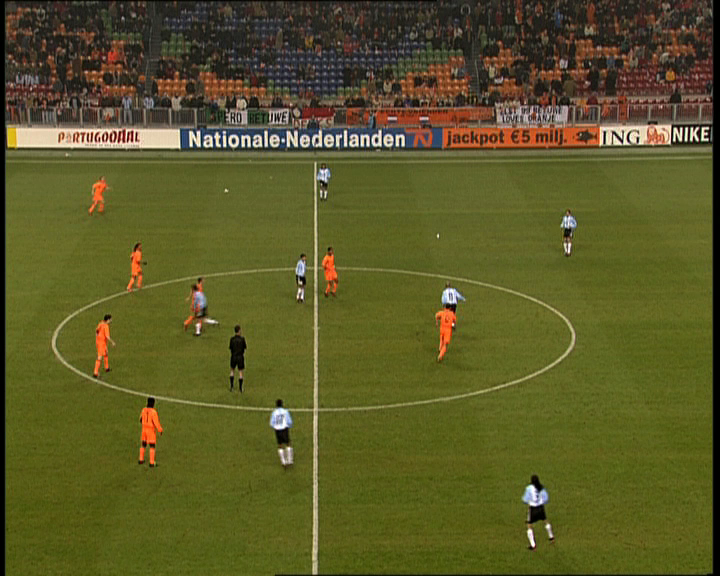
\includegraphics[width=0.4\textwidth]{img/footballocclusion.png}
    \label{fig:dataimages:football}}

  \subfigure[\texttt{ball1} movie, shot with dynamic lighting and showing the object in close-up.]{
    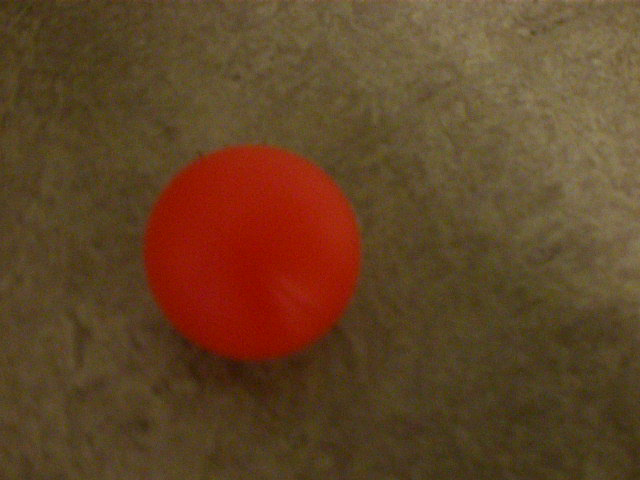
\includegraphics[width=0.35\textwidth]{img/bal1.png}
    \label{fig:dataimages:ball1}}
  \subfigure[\texttt{ball2} movie, with a consistently red ball, showing some background distractions in the corner.]{
    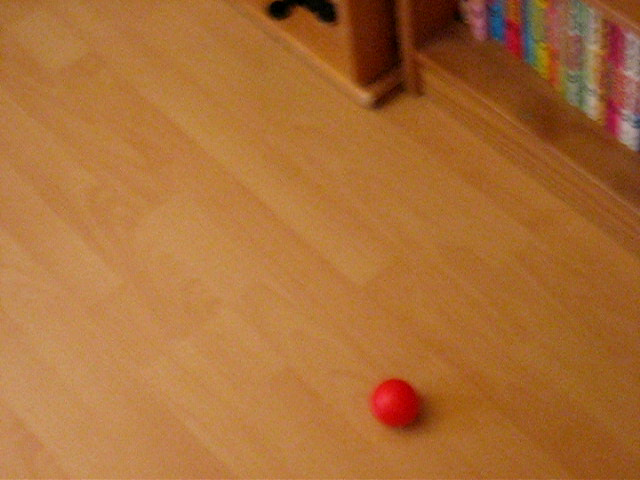
\includegraphics[width=0.35\textwidth]{img/bal2.png}
    \label{fig:dataimages:ball2}}
  \caption{Example still images from each of the movies used as data for evaluation.}
  \label{fig:dataimages}
\end{figure}


\section{Application}
\label{sec:application}
First we started to get familiar with Matlab, loading images, and doing matrix transformations on the images.
The most important step was to make our own colour space transformation for images.
The RGB2rgb function required special treatment, since when a pixel is black a divide-by-zero error may occur, and equation \ref{eq:rgb} becomes invalid for these values.
Because everything between black and white, and white itself, becomes grey, black should be grey also.
Since r+g+b is always 1 we need only to look at r and g, as the information for b is implicit in these values.
This reduces the dimensionality of the histogram to 2D.

Next was the creation of a histogram function for images.
Support for both 3D histograms (HSI/RGB) 2D histograms (rgb) and later 1D histograms (Hue) was implemented.
Three dimensional bins also allow for an easy visualisation of the histograms.
Using the histograms, a backprojection function was made as described in section \ref{sec:theory:histograms}
The result is a black and white image, where the dominant colors from the histogram are whiteish.

A method to indicate the similarity between histograms was first based on the Euclidian distance. Because we need to find a minimum distance, not a true distance, the square-root was left out.
The Bhattacharyya distance was also implemented.
Because it is applied to a discrete distribution, it differs slightly from the continuous definition of equation \ref{eq:bhattcoefficient}.
The coefficient is calculated as the pairwaise multiplication of each bin of both histograms.
Next the square root of each bin is taken, and summed.

To test the setup at this point, an object recognition function called `finding Nemo' was used.
We start with a cutout of Nemo, and replace the background with white.
This serves as the target image, from which an rgb histogram is can be made.
To increase the recognition, the grey values were removed from the histogram, since this is the dominant colour: the RGB background was white, and thus grey in the rgb image.
Then we do a backprojection with a new image where we want to find Nemo based on the histogram.
The result is a black and white image where colors similar to nemo are whitish and other colors are darker.
Finding the final object-shape is done by first increasing the contrast to acquire a binary image; next dilating and eroding to remove noise and create general shapes; last the built-in Matlab object segmentation was used to find groups of pixels and sort them by size.
The biggest blob then is the most likely Nemo candidate.
Figure \ref{fig:nemo} shows an example, where the biggest blob is presented by an enclosing rectangle.

\begin{figure}[ht]
  \centering
  \subfigure[The Nemo target image.]{
    \includegraphics[width=0.3\textwidth]{img/nemosearch.png}}
  \subfigure[A rectangle is drawn around the most likely position of Nemo.]{
    \includegraphics[width=0.45\textwidth]{img/nemofound.png}}
  \caption{Finding nemo using rgb and backprojection.}
  \label{fig:nemo}
\end{figure}

\subsection{Tracker}
\label{sec:application:tracker}
An exhaustive search that analyses an entire frame each iteration can be dismissed as even remotely feasible.
We adjusted the search to look only at a predefined area around the current location.
To further increase its speed, not all pixels are compared but only every other pixel.
The number of skipped pixels can be set using the parameter \texttt{searchStep}.
The exhaustive search does not use a kernel based histogram but only the original unweighted values, combined with the euclidian distance measure.
Given the initial position of the object, we step through the following frames, finding the location within the searcharea where the histogram is most similar to the target histogram.

Skipping pixels significantly improves the speed, but results in less accurate tracking.
It does not affect the sensitivity to loosing the object a lot, since the search area remains equal.
Increasing the search size makes the tracker less sensitive to fast movements, but may also introduce incorrect matchings with other similar objects and at the cost of reduced speed.

The mean-shift method implementation, and the main focus in the current system, was relatively straightforward.
It mainly involved combining all the single functions into one.
We calculate the new mean relative to the current position, so the initial new centre position is zero.
Then for every pixel, we add to the new centre the weighted pixels' histogram value, multiplied with the pixels' candidate position minus the candidate image size.
In effect, pixels left or up from the mean substract their weight from the new centre, while pixels right or up add to the new centre.
After all pixels are processed, the new centre directly is the new mean.

If an object `shifts' or `scales' out of the entire image, the current position is retained since a position outside the image is in principle undefined.

\subsection{Implementation}
\label{sec:application:implementation}
The input movies were converted to consecutive images in Portable Network Graphics (PNG) format, using \texttt{mplayer -vo png}.\footnote{See: \url{http://www.mplayerhq.hu/}}
This conversion is still affected by the video compression of the movie, but PNG employs a losless compression, retaining the original filming conditions as much as possible.

Table \ref{tab:parameters} shows the important parameter settings in the implementation and their possible values.

\begin{table}[ht]
  \centering
  \begin{tabular}{|l||l|l|}
    \hline
    Parameter name & Description & Possible values\\
    \hline
    \texttt{method} & Tracker method & \texttt{0}: mean-shift; \texttt{1}: brute force\\
    \texttt{scaling} & Use scaling & \texttt{0}: disabled; \texttt{1}: enabled\\
    \texttt{kernel} & Use Epanechnikov & \texttt{0}: disabled; \texttt{1}: enabled\\
    \texttt{bins} & Number of histogram bins & $\mathbb{N}$\\
    \texttt{colorSchema} & Colourspace & \texttt{RGB}, \texttt{RGBnorm}, \texttt{HSI}, \texttt{H}\\
    \texttt{searchStep} & Skipped pixels & $\mathbb{N}$\\
    \texttt{searchArea} & Searched area & $\mathbb{N}$\\
    \hline
  \end{tabular}
  \caption{Parameters used for tuning the performance.}
  \label{tab:parameters}
\end{table}

The object tracker can be run by executing the \texttt{main.m} function.
This takes no arguments, but all parameters should be set in the file itself.\footnote{Please take note to set the correct path to the directory containing a series of images.}


\section{Evaluation}
\label{sec:evaluation}
To evaluate the performance of the mean-shift tracker we chose three different evaluation measures.
First is the qualitative measure of visual interpretation.
This analysis is left for section \ref{sec:results}.
Two quantitative error measures are based on the Bhattacharyya distance and the path traveled by the object through the image dimensions.

\paragraph{Bhattacharyya distance} Because the Bhattacharyya distance describes how well a candidate image in a frame compares to the original target image, it also gives an indication of the performance of the tracker.
This measure is useful for a general analysis of the performance.
If the average distance (error) is low then the object was in clear view most of the time.

\paragraph{Path distance} When an object is tracked throughout a series of images, one would expect --or at least desire-- that the object would be tracked just as well in the reverse direction, using the first ending position as the new starting position.
We define the Path error as the distance between both the calculated object locations in one frame.
This error measure can give a good indication if an object was lost at some point, if the average and maximal distance differ significantly.
On the other hand, if the average an maximum (or minimum) are relatively equal, it is assumed that the same path was traveled twice and thus that the object was tracked correctly.\\

For both quantitative measures it is possible that a low error score occurs while the tracking itself was in fact unsuccessful.
For example, when an object is lost and found again twice in exactly the same way, the Path error will be erroneously low.
It is therefor always important to also visually confirm the results in some cases.

The tests were run using Matlab 7.6.0 for linux on a quadcore@2.6GHz CPU and 3GB RAM.
Although the code is not optimised for multicore processing, it does imply that all tests are run using an equal amount of CPU power (one core) and fully loaded in RAM.
The evaluation of the computational complexity is still not system independent, but it does make comparison of the results more viable.
Re-runs with the exact same evaluation settings have shown timing differences that remain within a 5\% margin.

Tables \ref{tab:error:ball2}, \ref{tab:error:ball1} and \ref{tab:error:football} show error measurements for \texttt{ball2}, \texttt{ball1} and \texttt{football} respectively.
All test were run using the mean-shift algorithm using the Epanechnikov kernel with scaling enabled, unless otherwise noted.

\begin{table}
  \centering
  \small
  \begin{tabular}{|l|l||l|l|l|l|}
    \hline
    Settings  & Binsize & Bhattacharyya & Path & Time (s)\\
    \hline
    rgb;      &  64    & 0.355/0.356/0.239/0.400 & 13.5/12/41     & 152\\
    Epan.     &  32    & 0.332/0.322/0.169/0.613 & 19.1/17/50.2   & 139\\
              &  16    & 0.379/0.366/0.205/0.603 & 20.3/16.4/62   & 212\\
    \hline
    rgb;      &  64    & 0.371/0.370/0.257/0.490 & 15.2/13/44.7   & 164\\
    no Epan.  &  32    & 0.368/0.366/0.213/0.531 & 48.9/29/197    & 189\\
              &  16    & 0.359/0.351/0.180/0.536 & 43.3/26/220    & 192\\
    \hline               
    H; Epan.  &  64    & 0.351/0.344/0.077/0.822 & 17.9/15.1/90.3 & 171\\
    \hline
  \end{tabular}
  \caption{Bhattacharyya (mean/median/min/max) and path (mean/median/max) error scores for \texttt{ball2}. Settings include the colourspace and the use of the Epanechikoc kernel or not.}
  \label{tab:error:ball2}
\end{table}

\begin{table}
  \centering
  \small
  \begin{tabular}{|l|l||l|l|l|l|}
    \hline
    Settings  & Binsize & Bhattacharyya & Path & Time (s)\\
    \hline
    rgb       &  32    & 0.761/0.961/0.320/1 & 376/392/589 & 49\\
              &  16    & 0.706/0.946/0.155/1 & 361/380/590 & 49\\
    \hline               
    H         &  64    & 0.699/0.919/0.132/1 & 342/373/586 & 49\\
              &  16    & 0.776/0.783/0/1     & 213/265/442 & 49\\
    \hline
  \end{tabular}
  \caption{Bhattacharyya (mean/median/min/max) and path (mean/median/max) error scores for \texttt{ball1}. Settings include the colour space.}
  \label{tab:error:ball1}
\end{table}

\begin{table}
  \centering
  \small
  \begin{tabular}{|l|l||l|l|l|l|}
    \hline
    Settings  & Binsize & Bhattacharyya & Path & Time (s)\\
    \hline
    rgb       &  64    & 0.651/0.644/0.524/0.898 & 4.80/4.12/15.8  & 39\\
              &  32    & 0.541/0.530/0.362/0.783 & 5.25/4.47/17.5 & 38\\
              &  16    & 0.481/0.490/0.260/0.713 & 5.6/5.1/21.8 & 39\\
    \hline
    H         &  64    & 0.568/0.527/0.283/0.963 & 287/397/633 & 36\\
              &  32    & 0.521/0.477/0.240/0.916 & 283/296/720 & 38\\
              &  16    & 0.429/0.417/0.200/0.846 & 208/295/422 & 36\\
    \hline
    rgb; Exh. Search & 16 & 0.402/0.4/0.226/0.619 & 99.8/101/160 & 72\\
    \hline
  \end{tabular}
  \caption{Bhattacharyya (mean/median/min/max) and path (mean/median/max) error scores for \texttt{football}. Settings include the colour space, and in the last row the use of an exhaustive search instead of mean-shift.}
  \label{tab:error:football}
\end{table}


\section{Results}
\label{sec:results}
If we look at the scores a good overall performance is achieved with normalised RGB (rgb) and 64 bins.
Examples of the tracking done with these evaluation settings are available online for all three movies: \href{http://www.youtube.com/watch?v=Rdj2X9cl9d8}{football}, \href{http://www.youtube.com/watch?v=bXcCzgcYsHU}{ball1} and \href{http://www.youtube.com/watch?v=39qQH3T52Nc}{ball2}.
These movies show that the correct object is tracked throughout the entire image sequence.
Not shown in the evaluative tables is a different object in the \texttt{football} movie, where a player is partly occluded by a player of the other team, i.e. of a different colour.
This occlusion is resolved well resulting in a comparable evaluation score.

With the \texttt{ball2} movie the average Bhattacharyya score is similar to the other tests, but the maximum score is significantly lower.
It should be noted that the Bhattacharyya scores are actually worse when looking at the \texttt{football} movie.
The Path scores on the other hand are consistently lower for all movies.

In terms of computational complexity there is little difference, except that mean-shift is considerably faster than exhaustive search.
An interesting point is that in the \texttt{ball2} movie a binsize of 16 appears a bit slower than a binsize of 64, even though it requires less computations per histogram comparison.
Possibly this can be ascribed to the iterative process of the mean-shift, meaning that a smaller binsize requires more shifting steps to find the new position.

Still the performance of the Hue is not so different from normalised RGB for the ball movies.
The \texttt{ball1} movie performs badly on all the test shown in table \ref{tab:error:ball1}.\footnote{Please note that the scores for the settings with which the well performing \texttt{ball1} youtube movie was made, are not included, due to some technical difficulties.}
It is hard to ascribe a better performance to either normalised RGB or Hue.

Another indication of problems is also suggested in both the ball movies.
After scaling the position of the object is based not on the entire object, but on an part of the object including some of the background.
This indicates that with the current methods and features it is not possible to compute a complete object description.
With different parameter settings the scores decrease dramatically, which can be shown to come from the tracker losing the object.
Figure \ref{fig:ballgraphs} shows the Path error plotted for each frame in two different \texttt{ball2} settings.

\begin{figure}[ht]
  \centering
  \subfigure[\texttt{ball2} Path error, showing good overall performance.]{
    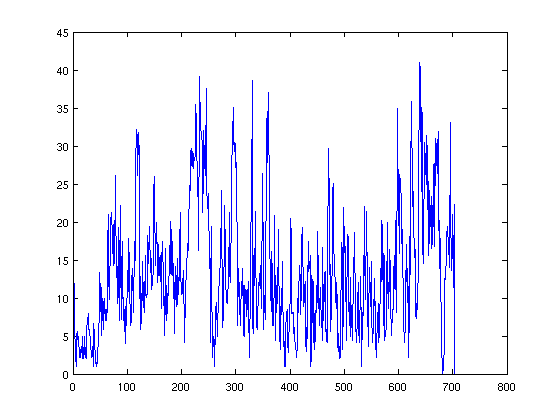
\includegraphics[width=0.45\textwidth]{img/bal2goed.png}
    \label{fig:ballgraphs:good}}
  \subfigure[\texttt{ball2} Path error, showing the object was (relatively) lost due to scaling problems.]{
    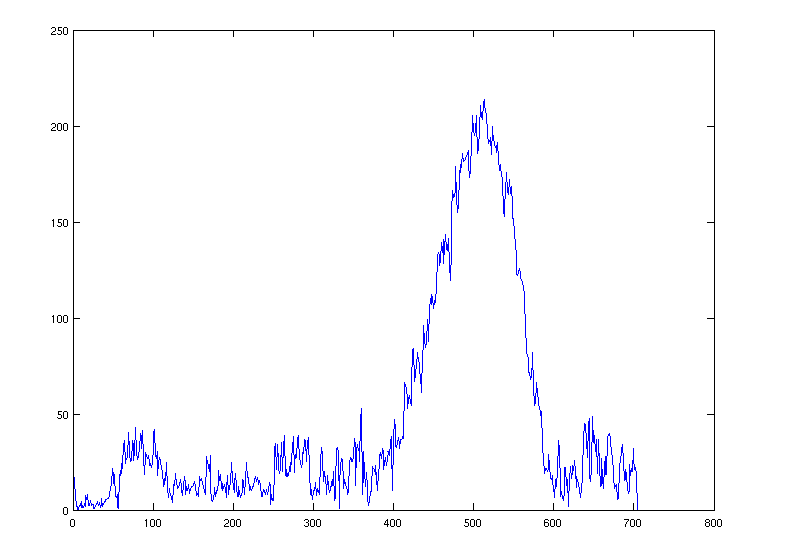
\includegraphics[width=0.45\textwidth]{img/bal2slecht.png}
    \label{fig:ballgraphs:bad}}
  \caption{Path error plots for the \texttt{ball2} movie.}
  \label{fig:ballgraphs}
\end{figure}


\section{Discussion}
\label{sec:discussion}
One of the unresolved questions when using the mean-shift algorithm is the choice of a specific colour space.
An automated solution could be to utilise a combination, and for each frame use the shift of the colour that has the lowest Bhattacharyya distance.

Second, scaling is still quite problematic.
In our case when an object is scaled, the tracker often prefers the edge of the object and not the complete object.
This can be explained by the fact that the initial selection of the object often includes some of the background.
Hence when an object becomes larger, the best matching histogram can very well be a small image patch at the border of the object.
The Epanechnikov kernel should compensate the fact that the main object now resides on a border rather than in the middle, but apparantly it does not.
It might be possible to experiment further with the Epanechnikov kernel to increase performance.
A second possibile explanation is that the perceived colour histogram of the object changes when it is scaled.
In this case, the colour model is not invariant enough, leading to a solution of the first problem mentioned in this section.

Third, after an object is lost, the tracker becomes useless.
Some sort of failure resolving can be built in.
When the Bhattacharyya coefficient between the target and candidate becomes too high, a global search could be done, similar to the `finding nemo' object recognition.
The biggest object similar to the original histogram is most likely the object we are looking for.
This is not of course not a definite solution.
In the ball movies, this could work very well since there is only one object in a relatively homogeneous background.
With the football movie on the other hand, there are multiple possible objects.
Even if we do a breadth-first exhaustive search starting at the last known location --searching until a Bhattacharyya score below some threshold is found-- there is no guarantee that the original object will be retrieved.
However, it is a good example of how some technique that is not generally feasible (like exhaustive search) can be a good alternative in some specific cases.
Even more so, if the exhaustive search fails to find a reasonable object, it could trigger an `object lost' response that can be just as valuable in object tracking as the actual tracking itself.


\section{Conclusion}
\label{sec:conclusion}
We investigated the problem of object tracking in moving images.
The current approach uses the mean-shift algorithm, combined with colour as feature space.
A visual evaluation on three sample movies suggests that this approach is indeed feasible.
Objects can be correctly tracked in near real-time, under changing conditions including illumination, occlusion and scaling.

Problems can also be identified, showing that robustness is not yet optimal and that a general application will require improvements.
Without tuning the starting parameters like the initial object area, and the specific colourspace and binsize, performance can decrease significantly.
Some suggestions for improvement include automating and optimising the choice for colourspace and actively searching for the object when it appears lost.


% Simple biblio for this report.
\begin{thebibliography}{1}
  \bibitem{surveycolor} Th. Gevers, ``Color in Image Search Engines,'' {\it Principles of Visual Information Retrieval,} ed. M. Lew, Springer Verlag, February 2001.
  \bibitem{kernelbased} D. Comaniciu, V. Ramesh, and P. Meer, ``Kernel-Based Object Tracking,'' {\it IEEE trans. on Pattern Recognition and Machine Intelligence,} May 2003, vol. 25, number 5, pp. 564-578.
\end{thebibliography}


\end{document}
